\documentclass{article}

\usepackage[submission]{colm2026_conference}
\usepackage{microtype}
\usepackage{hyperref}
\usepackage{url}
\usepackage{booktabs}
\usepackage{graphicx}
\usepackage{amsmath}
\usepackage{lineno}

\definecolor{darkblue}{rgb}{0, 0, 0.5}
\hypersetup{colorlinks=true, citecolor=darkblue, linkcolor=darkblue, urlcolor=darkblue}
\Urlmuskip=0mu plus 2mu\relax

\title{\method: Source-Private Candidate-Transfer Packets under Destructive Controls}

\author{Anonymous authors\\Paper under double-blind review}

\newcommand{\method}{LatentWire}
\newcommand{\arc}{ARC-Challenge}
\newcommand{\obqa}{OpenBookQA}

\begin{document}

\ifcolmsubmission
\linenumbers
\fi

\maketitle

\begin{abstract}
Multi-model language systems usually communicate by emitting text or by sharing internal state such as KV caches. Text is portable but exposes source outputs; cache sharing is information-rich but moves and exposes dense model state. We study a deliberately narrower interface: can a frozen source model send a byte-scale, source-private packet that helps a frozen receiver on public multiple-choice reasoning tasks without sending source text, hidden states, KV cache, source logits, or labels? We present \method, a packet protocol and evaluation framework with explicit byte accounting, a source-private threat model, and destructive controls for source-choice, wrong-row, coordinate-shuffle, same-budget text, and cross-family shortcuts. On \arc{} test, an 8-byte payload / 11-byte framed packet reaches 0.344 accuracy across 10 seeds, above target-only 0.265 and same-budget structured text 0.300; on \obqa{} test, a 3-byte / 6-byte packet reaches 0.378 across 5 seeds, above target-only 0.276 and same-budget text 0.350. The decisive audit is also limiting: explicit source-index communication reaches 0.346 on \arc{} and 0.378 on \obqa{}, so the current positive is narrow source-candidate transfer, not evidence synthesis beyond the source or a method that beats selected-candidate communication. We also report that a Phi-3 cross-family source fails and that simple cached connector repairs do not close the gap. The workshop contribution is a reproducible packet-transfer result, a strict falsification protocol, and a systems boundary artifact: headline packets are 6--11 framed bytes, while dense KV/cache-transfer regimes begin hundreds to thousands of bytes per token under our accounting. We do not claim solved latent communication, C2C superiority, or native GPU latency/HBM/energy wins.
\end{abstract}

\section{Introduction}

Future language-model systems will often use more than one model: a cheap model may screen candidates, a specialist may inspect hard cases, and a stronger receiver may combine evidence. The simplest interface is text. Recent cache-level systems instead communicate through model internals, such as fused or selectively shared KV caches~\citep{Fu2025C2C,Shi2025KVComm}. These approaches are powerful, but they couple communication to large hidden-state objects and serving substrates.

This paper asks whether a much smaller interface can carry useful source-side candidate evidence. In our setting, both models see the same public question and answer choices. The source performs private computation over those choices. The only communicated object is a short byte packet; the receiver never sees source text, source logits, source hidden vectors, KV cache, or the answer key. This is a side-information problem in the spirit of distributed source coding~\citep{Slepian1973Noiseless,Wyner1976RateDistortion}: the receiver already has the public prompt and its own computation, so the packet should carry only the source evidence that is useful at the decoder. The scientific contribution is therefore not just a packet row, but a reviewable protocol for asking whether such rows survive the controls that usually create false positives.

Our strongest current result is deliberately scoped. On \arc{} and \obqa{}~\citep{Clark2018ARC,Mihaylov2018OpenBookQA}, same-family Qwen2.5 packet transfer~\citep{Yang2025Qwen25} improves over target-only and same-budget text controls. However, a strict Phi-3 source-family replacement~\citep{Abdin2024Phi3} fails, and additional connector repairs fail on the available TinyLlama/Qwen cached artifacts. This boundary matters: the paper is not claiming solved cross-family latent communication.

The contributions are:
\begin{itemize}
\item A byte-scale, source-private packet protocol and threat model for multiple-choice candidate transfer with no source text, hidden vector, KV cache, source-logit, or gold-label exposure.
\item A strict evaluation suite that combines target-only, same-budget text, source-index/rank, coordinate-shuffle, wrong-row, same-source-choice, cross-family, and cached-connector controls.
\item Controlled narrow positives on \arc{} and \obqa{} with seed repeats and paired uncertainty, accompanied by an explicit source-index audit showing that the current effect is mostly source-choice preserving.
\item A failure-boundary analysis showing that Phi-3 cross-family transfer and simple cached connector repairs fail, so broad latent-language and cross-family claims are unsupported.
\item A systems accounting artifact comparing raw, framed, cacheline-rounded, and dense KV/cache byte regimes while separating measured packet objects from analytical byte floors and future native GPU measurements.
\end{itemize}

This is useful even with a narrow positive because it separates three questions that are often conflated: whether a compact private packet can help, whether it carries more than the source's preferred answer, and whether it is cheaper or less exposing than dense state transfer. The current answer is positive for the first question, negative for the second, and accounting-only for the third. That scoped result is the paper's intended workshop contribution.

\paragraph{Where the current result is useful.}
The current method is most plausible for same-family cascades, privacy-preserving specialist-to-router hints, and bandwidth-limited candidate reranking where sending source generations, logits, hidden states, or KV cache is undesirable. It is not yet a method for open-ended generation, heterogeneous cross-family collaboration, or reasoning synthesis beyond the source model's selected candidate.

\begin{figure}[t]
  \centering
  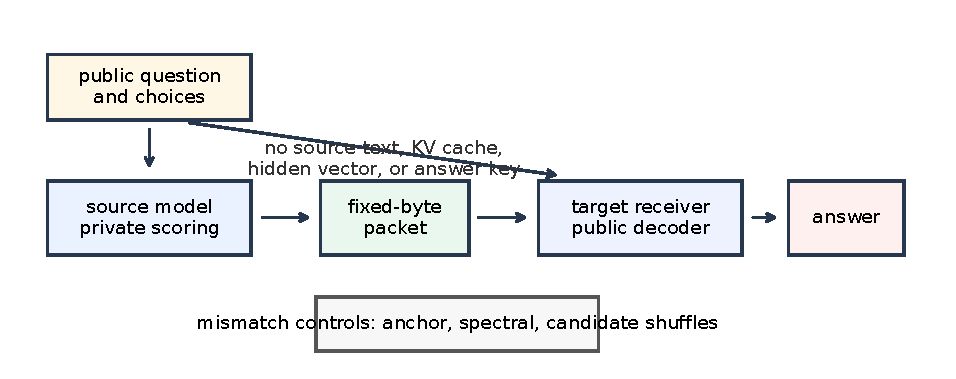
\includegraphics[width=0.96\linewidth]{figures/protocol_diagram.pdf}
  \caption{\method{} protocol. Both sides receive the public task. The source privately scores candidates and emits only a fixed-byte packet. The receiver decodes the packet with a public basis and its own side information. Destructive controls scramble the shared coordinate system or candidate relation.}
  \label{fig:protocol}
\end{figure}

\section{Source-private packet transfer}

Let a public multiple-choice instance be $x=(q,c_1,\ldots,c_m)$ with answer choices $c_i$. A source model $S$ and receiver $R$ both observe $x$, but only $S$ computes the source-side private evidence $e_S(x)$. A packet encoder emits
\[
z = E(e_S(x), x), \qquad |z| \leq B \text{ bytes}.
\]
The receiver predicts
\[
\hat{y} = D_R(x,z),
\]
where $D_R$ may use public task features and the receiver's own state, but may not access source text, source hidden states, source KV cache, source logits, or answer labels.

We evaluate a packet only if it beats three surfaces: target-only $D_R(x,\emptyset)$, a same-budget structured text control, and destructive controls that preserve superficial packet size but destroy the intended source-receiver relation. We also audit explicit source-index, source-label-text, source-rank-code, and entropy-matched random-index baselines. We report seed repeats and paired bootstrap lower bounds. This matters because a packet can be useful while mostly preserving the source's selected candidate; such a result is source-private transfer, not proof of a shared latent language, reasoning beyond the source endpoint, or compression beyond a one-byte selected-candidate channel.

\paragraph{Threat model.}
The packet channel is source-private but not source-oblivious. The sender may privately compute over the public prompt and answer choices, then transmit only a bounded byte string. The receiver may use that byte string, the public prompt, and its own computation. The receiver may not observe source generations, chain-of-thought, hidden states, KV cache, logits, score vectors, or labels. A passive packet observer sees only the packet bytes and framing, not source internals or text; however, the current packet can still leak the source's preferred candidate. We therefore distinguish privacy of source state from secrecy of source choice. A method fails the current workshop claim if its apparent gain is matched by a target-only cache effect, same-budget visible text, explicit source-index/rank/score communication, wrong-row transfer, or answer leakage.

\paragraph{Control suite.}
Table~\ref{tab:controls} lists the reviewer-facing controls used to interpret the reported rows. The suite is intentionally stronger than the headline claim: several controls are designed to collapse methods that only copy the source's preferred answer choice.

\begin{table}[t]
  \centering
  \scriptsize
  \setlength{\tabcolsep}{3pt}
  \begin{tabular}{p{0.22\linewidth}p{0.36\linewidth}p{0.31\linewidth}}
    \toprule
    Control family & What it tests & Current role \\
    \midrule
    target-only / zero-source & target-cache or no-packet effects & required baseline \\
    same-budget visible text & whether text at the same byte budget suffices & required baseline \\
    source-index / rank / score & selected-candidate shortcuts & main claim boundary \\
    wrong-row / row shuffle & row-specific source causality & destructive control \\
    same-source-choice wrong-row & source-choice-only transfer & hardening control \\
    anchor/bin/coordinate shuffle & shared-coordinate dependence & mechanism control \\
    candidate roll/derangement & answer-order artifacts & destructive control \\
    source-family substitution & cross-family generality & falsification control \\
    cached connector repair & easy learned receiver rescue & negative diagnostic \\
    \bottomrule
  \end{tabular}
  \caption{Control suite. The workshop claim requires packet utility to be interpreted through these controls; the current positive is explicitly bounded by source-index and source-family failures.}
  \label{tab:controls}
\end{table}

\section{Public-coordinate packets}

The current \arc{} implementation uses a public train-anchor chart. For each candidate, we compute a public relative-coordinate feature against a frozen set of training anchors, then project that feature into a low-frequency orthonormal DCT-II spectral basis. The packet is a sparse signed syndrome in this shared coordinate system. The receiver scores candidate compatibility with the packet in the same public basis, combining the packet evidence with receiver-side candidate information.

The design is related to relative representations~\citep{Moschella2023Relative}: anchors provide a coordinate system less tied to raw hidden dimensions. Our use is narrower. We do not claim zero-shot latent stitching or global representation alignment; we use a public basis to define a tiny task packet. Random shared anchors work nearly as well as semantic anchors in the current hashed \arc{} implementation, so the correct interpretation is shared coordinate agreement, not semantic anchor names.

\obqa{} uses the same packet-evaluation contract at a smaller 3-byte budget. Across both tasks, the source-choice cache is answer-key-forbidden: the source sees public questions and choices, not labels. The packet is evaluated on frozen test slices after validation selection.

\section{Main results}

Table~\ref{tab:main} and Figure~\ref{fig:accuracy} summarize the current positive evidence and the source-index audit. The \arc{} row uses 10 packet/control seeds and 2000 paired bootstrap samples per seed on 1172 test examples. The \obqa{} row uses 5 seeds on the 500-example test slice. The source-index audit is generated by reconstructing the same packet rows and adding explicit source-index, source-label-text, source-rank-code, and entropy-matched random-index baselines.

\paragraph{Reproducibility card.}
All headline rows are frozen test-slice evaluations. The \arc{} row uses Qwen2.5-family source/target caches, 10 seeds, and 2000 bootstrap samples; the \obqa{} row uses the same source-private contract with 5 seeds and 500 bootstrap samples; the source-index audit reruns the same frozen prediction surfaces with explicit index/rank/label baselines. Exact input paths, hashes, scripts, and rerun status are listed in the artifact manifest and regenerated by the COLM\_v3 review-packet script.

\begin{table}[t]
  \centering
  \small
  \setlength{\tabcolsep}{3.8pt}
\begin{tabular}{llrrrrrrrr}
    \toprule
    Benchmark & split & bytes & seeds & src & packet & target & text & pkt-src & pkt-text \\
    \midrule
    \arc{} & test, 1172 & 8/11 & 10 & 0.346 & 0.344 & 0.265 & 0.300 & -0.008 & +0.025 \\
    \obqa{} & test, 500 & 3/6 & 5 & 0.378 & 0.378 & 0.276 & 0.350 & -0.006 & +0.000 \\
    \bottomrule
  \end{tabular}
\caption{Main audit rows. ``Bytes'' reports payload/framed bytes. ``Src'' is explicit answer-key-forbidden source-index accuracy before packet decoding. ``Text'' is the same-budget structured text control. ``Pkt-src'' and ``pkt-text'' are minimum paired-bootstrap 95\% lower bounds for packet minus source-index and packet minus same-budget text. Packet-minus-target lower bounds are +0.038 on \arc{} and +0.046 on \obqa{}.}
  \label{tab:main}
\end{table}

\begin{figure}[t]
  \centering
  
\includegraphics[width=0.92\linewidth]{figures/accuracy_overview.pdf}
  \caption{Packet accuracy against target-only and same-budget structured text controls. Error bars show the lower paired-bootstrap lift above target-only; upper uncertainty is omitted for readability because the gate is one-sided.}
  \label{fig:accuracy}
\end{figure}

On \arc{}, the matched Fourier/anchor-syndrome packet reaches 0.344 mean test accuracy with minimum seed accuracy 0.342. The answer-key-forbidden source index itself reaches 0.346, and packet predictions match the source-selected candidate at 0.995 mean rate across seeds. Anchor-ID shuffle, anchor-value shuffle, and spectral-bin permutation controls all fail in 0/10 seeds and collapse near target-only. The random shared-anchor diagnostic passes, which weakens any claim that named anchors are semantically special, but strengthens the claim that a shared public coordinate chart is the relevant mechanism.

On \obqa{}, the 3-byte packet reaches 0.378--0.380 across seeds. The explicit source-index baseline reaches 0.378, and the packet follows the source index at 0.999 mean rate. The largest candidate-derangement control accuracy is 0.212, and the packet beats same-budget structured text in mean by +0.028, with a paired lower bound of +0.000. This second task reduces the risk that the result is only an \arc{} artifact, but it confirms the same boundary: the current method is source-choice preserving and same-family, not cross-family latent reasoning.

The practical readout is an evidence ladder rather than a single win/loss row. The packets beat target-only and same-budget text on the headline rows; coordinate and candidate-destructive controls prevent treating the result as random packet regularization; explicit source-index/rank controls prevent overstating the mechanism. In framed-byte terms, the target-only lift is $0.079/11=0.0072$ accuracy per byte on \arc{} and $0.102/6=0.0170$ accuracy per byte on \obqa{}. Those rates are useful for comparing packet regimes, but they are not evidence that the current packet is better than a direct selected-candidate code.

\paragraph{Claim boundary.}
The current packet does not improve over explicit source-index communication: source-index reaches 0.346 on \arc{} and 0.378 on \obqa{}, while the packet reaches 0.344 and 0.378. We therefore claim source-private fixed-byte candidate transfer under destructive controls, not compression beyond a selected-candidate channel.

\paragraph{Breadth audits.}
We keep additional model and benchmark breadth in the reviewer packet rather than turning every diagnostic into a headline claim. A frozen benchmark-selection gate also records HellaSwag validation-1024~\citep{Zellers2019HellaSwag} as a positive bounded validation diagnostic, CommonsenseQA~\citep{Talmor2019CommonsenseQA} as target-positive but same-byte-text saturated, and SciQ~\citep{Welbl2017SciQ} as a source-private bridge contract with no positive packet row yet. A separate latest-model emitter audit covers Qwen3.5, Gemma 4, Granite 3.3, and OLMo-2 source-packet behavior on a synthetic hidden-repair benchmark. These rows improve reviewer visibility into breadth and failure modes, but they are not used to strengthen the main \arc{}/\obqa{} claim.

\begin{table}[t]
  \centering
  \scriptsize
  \setlength{\tabcolsep}{4pt}
  \begin{tabular}{lrrrrl}
    \toprule
    Benchmark & seeds & pkt-target & pkt-text & pkt-source & provenance \\
    \midrule
    \arc{} & 10 & +0.038 & +0.025 & -0.008 & frozen test, hash-audited \\
    \obqa{} & 5 & +0.046 & +0.000 & -0.006 & frozen test, hash-audited \\
    \bottomrule
  \end{tabular}
  \caption{Uncertainty summary for the main audit rows. Values are paired-bootstrap 95\% lower bounds for packet accuracy minus the named comparator. The zero lower bound against same-budget text on \obqa{} is intentionally visible: that row is a narrow secondary positive, not a strong text-baseline separation.}
  \label{tab:uncertainty}
\end{table}

\begin{figure}[t]
  \centering
  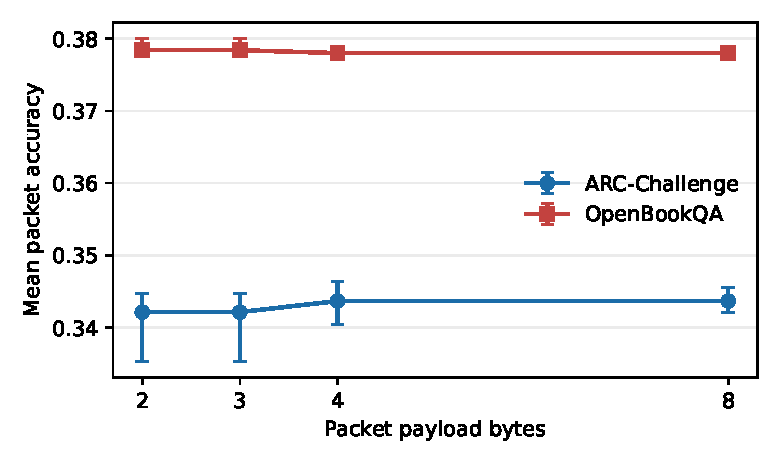
\includegraphics[width=0.86\linewidth]{figures/rate_curve.pdf}
  \caption{Payload-rate curve from the source-index audit. Packet payloads below 2 bytes are unsupported by the current sparse signed encoder; the 1-byte source-index baseline is reported separately in Table~\ref{tab:main}.}
  \label{fig:rate}
\end{figure}

\section{Falsification and failure decomposition}

The most important negative result is the Phi-3 source-family replacement. We keep the same \arc{} packet budget, public basis, seed count, and bootstrap budget, but replace the Qwen source-choice cache with a Phi-3 source. The packet no longer passes. On the full \arc{} test slice, the Phi-3 packet reaches 0.244 versus target-only 0.265. On the stricter Qwen-disagreement slice, where the alternate source and Qwen source disagree, the Phi-3 packet reaches 0.200 versus 0.340 for the Qwen-substituted packet.

\begin{table}[t]
  \centering
  \small
  \setlength{\tabcolsep}{3.4pt}
  \begin{tabular}{llrrrrrl}
    \toprule
    Source & surface & n & packet & target & text & ref. pkt & blocker \\
    \midrule
    Phi-3 & full test & 1172 & 0.244 & 0.265 & 0.232 & -- & source quality \\
    Phi-3 & Qwen-disagree & 833 & 0.200 & 0.273 & 0.203 & 0.340 & source quality \\
    TinyLlama & Qwen-disagree & 473 & 0.269 & 0.268 & 0.258 & 0.317 & family mismatch \\
    Qwen2.5-1.5B & full test & 1172 & 0.442 & 0.265 & 0.401 & -- & val incomplete \\
    \bottomrule
  \end{tabular}
  \caption{Cross-family and source-family diagnostics. ``Ref. pkt'' is the Qwen-substituted packet on disagreement rows. Qwen2.5-1.5B is encouraging but same-family and validation-incomplete, so it is not a headline cross-family claim.}
  \label{tab:falsification}
\end{table}

The failure decomposition separates three causes: source endpoint quality, packet corruption, and common-feature mismatch. For Phi-3, packet predictions follow the Phi-3 source choice at 0.997, but the source itself is below the target. For TinyLlama, packet fidelity is also high, but the source-family mismatch causes the disagreement-slice packet to lose to Qwen-substituted packets. For Qwen2.5-1.5B, the source is stronger and the packet is useful on frozen test, but the validation disagreement gate is incomplete. Across these rows, the packet mostly transports the source-selected candidate through the public coordinate basis. The source-index audit in Table~\ref{tab:main} closes one obvious reviewer question: the current packet does not beat a direct selected-candidate code. The next research gate is therefore a richer common-feature connector or calibrated source-score packet that can improve beyond packet-only source choice.

We also tested cached learned repairs on the available local artifacts. A candidate-syndrome connector that sees packet and score-shape features reaches 0.288 versus 0.317 for Qwen-substituted packets on frozen TinyLlama/Qwen disagreement rows. A one-hidden-layer MLP over cached TinyLlama hidden/query summaries reaches 0.232, below Qwen-substituted packets, cached Tiny packets, target-only, and same-budget text. These negatives are useful: simple cached score geometry and mean hidden/query summaries do not explain the remaining oracle headroom.

\section{Systems boundary}

The systems contribution is byte/exposure accounting, not native serving throughput. Figure~\ref{fig:systems} compares framed packet bytes with one-token KV/cache-state accounting floors from neighboring systems and quantization methods. \method{} sends 6--11 framed bytes on the two headline rows. A one-token 1-bit-per-KV-element accounting floor is 768 bytes in our model-configuration accounting; the largest headline packet is therefore 69.8x smaller than that floor. C2C-style cache transfer, KVComm-style selective sharing, and serving substrates such as vLLM/PagedAttention and SGLang operate on KV/cache objects rather than task-level packets~\citep{Fu2025C2C,Shi2025KVComm,Kwon2023vLLM,Zheng2023SGLang}. KV quantization work reduces cache bytes but still communicates or stores model state~\citep{Zandieh2024QJL,Liu2024KIVI,Hooper2024KVQuant,Zandieh2025TurboQuant}.

We label packet-object bytes as measured/accounted local artifacts and dense-state rows as analytical or literature-derived byte floors. This distinction is important: the current data support privacy/exposure and byte-budget comparisons, but not claims about GPU latency, HBM traffic, energy, or serving throughput.

\begin{figure}[t]
  \centering
  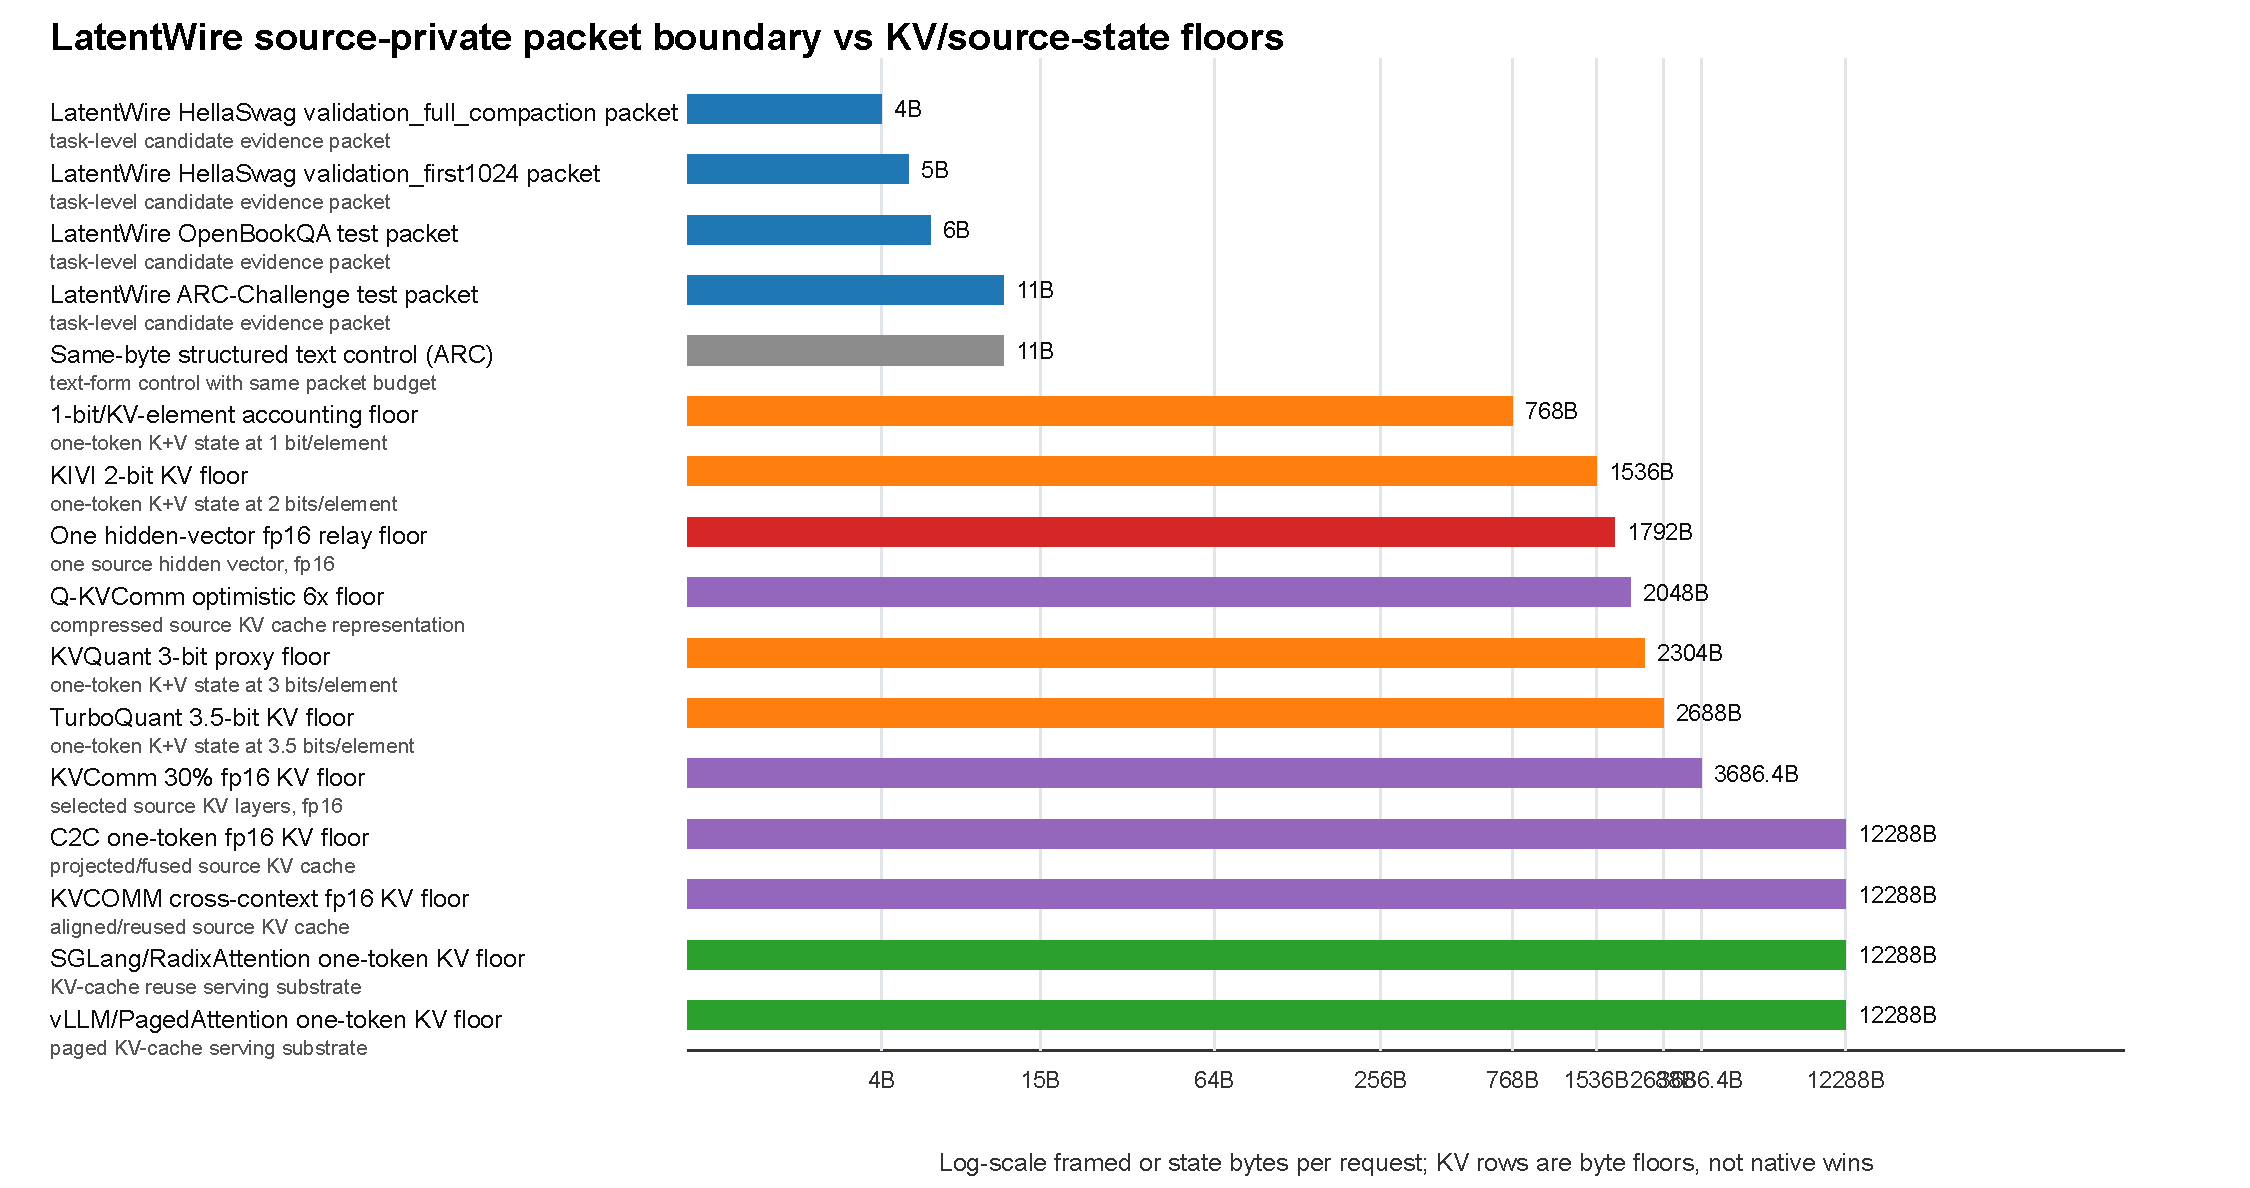
\includegraphics[width=0.95\linewidth]{figures/systems_boundary.pdf}
  \caption{Boundary-byte accounting. Packet rows are measured task-packet objects. KV/cache rows are lower-bound floors or neighboring serving substrates, not native speed comparisons.}
  \label{fig:systems}
\end{figure}

\begin{table}[t]
  \centering
  \small
  \setlength{\tabcolsep}{3.8pt}
  \begin{tabular}{lrrlll}
    \toprule
    Method & raw & framed & text & KV/hidden & claim status \\
    \midrule
    \method{} \obqa{} packet & 3B & 6B & no & no & local positive \\
    \method{} \arc{} packet & 8B & 11B & no & no & local positive \\
    Same-byte text control & 8B & 11B & yes & no & control only \\
    1-bit/KV-element floor & 768B & 768B & no & KV & floor only \\
    KIVI 2-bit KV floor & 1536B & 1536B & no & KV & floor only \\
    C2C one-token KV floor & 12288B & 12288B & no & KV & native pending \\
    \bottomrule
  \end{tabular}
\caption{Exposure classes. Packet rows are measured/accounted local communication objects. KV/cache rows are analytical byte floors or native-pending baselines. The paper-ready systems claim is object size and source-exposure accounting, not GPU throughput, TTFT, TPOT, HBM, energy, or C2C superiority.}
  \label{tab:systems}
\end{table}

\section{Related work}

\textbf{Latent and relative representation communication.} Relative representations use similarities to anchors to enable latent-space communication under invariances~\citep{Moschella2023Relative}. Sparse autoencoder work motivates interpretable feature coordinates~\citep{Cunningham2023SAE}, while feature-space universality work suggests that some features can be related across models~\citep{Engels2024SAEUniversality}. Crosscoders, transcoders, and activation-transfer methods are natural future sources of interpretable packet atoms or dense communication baselines. SAEBench provides evaluation machinery for sparse autoencoders~\citep{Karvonen2025SAEBench}, but these works do not by themselves provide a byte-counted packet protocol or task-level evidence transfer result under source-choice controls.

\textbf{Prompt compression and learned prefixes.} Prefix tuning and gist tokens learn continuous or discrete prompt-like interfaces within language models~\citep{Li2021Prefix,Mu2023Gist}; text-compression systems such as LLMLingua and LongLLMLingua are stronger visible-text baselines for future work~\citep{Jiang2023LLMLingua,Jiang2023LongLLMLingua}. \method{} differs because the communicated object is an opaque byte packet decoded by a public receiver, not a learned soft prompt injected into one target or a compressed visible prompt. Query-bottleneck connectors such as BLIP-2's Q-Former show that learned bottlenecks can bridge frozen model families across modalities~\citep{Li2023BLIP2}; our failed cached hidden/query summaries suggest that a true tokenwise query-bottleneck is the right future branch, but it is not closed here.

\textbf{Cache communication and systems.} Cache-to-cache and selective KV-sharing systems communicate richer internal state and are the closest competitors for model-to-model communication~\citep{Fu2025C2C,Shi2025KVComm}. vLLM and SGLang improve serving through KV-cache management and reuse~\citep{Kwon2023vLLM,Zheng2023SGLang}. KV quantizers such as QJL, KIVI, KVQuant, and TurboQuant reduce state cost but remain state-transfer or state-storage techniques~\citep{Zandieh2024QJL,Liu2024KIVI,Hooper2024KVQuant,Zandieh2025TurboQuant}. Table~\ref{tab:baseline-matrix} summarizes how these baselines differ from \method{}. Our current systems result is a boundary artifact against these state objects, not a native throughput win.

\begin{table}[t]
  \centering
  \scriptsize
  \setlength{\tabcolsep}{3pt}
  \begin{tabular}{p{0.17\linewidth}p{0.17\linewidth}p{0.31\linewidth}p{0.27\linewidth}}
    \toprule
    Regime & Example & Object crossing interface & Difference from \method{} \\
    \midrule
    dense cache fusion & C2C & projected source KV cache & high-bandwidth, source-state exposing \\
    selective KV sharing & KVComm & selected KV pairs/layers & cache-level, native pending \\
    KV compression & KV quantizers & compressed KV/cache state & shrinks dense state, not source-private task packets \\
    serving substrate & vLLM/SGLang & KV reuse and memory management & runtime baseline, not communication protocol \\
    prompt/prefix compression & prefix/gist tokens & prompt-like tokens or parameters & not source-private model-to-model evidence \\
    local shortcut baselines & source-index/rank/score & selected answer or score sketch & must be beaten for stronger claims \\
    \bottomrule
  \end{tabular}
  \caption{Related-work and baseline matrix. \method{} is positioned as low-byte source-private packet transfer with destructive controls, not as a replacement for dense cache fusion or serving-runtime optimization.}
  \label{tab:baseline-matrix}
\end{table}

\section{Limitations and next gate}

The main limitation is scope. The positive results are same-family/source-cache results on public multiple-choice tasks, and the packet largely preserves the source's selected candidate. We therefore do not claim to beat explicit source-index communication, source-score quantization, or calibrated source-choice baselines; those are required before a stronger compression claim. Phi-3 cross-family replacement fails, TinyLlama common-feature repair fails, and a true cross-family learned query-bottleneck remains future work. We also do not claim superiority over C2C, KVComm, QJL, KIVI, TurboQuant, vLLM, or SGLang in native serving metrics. Those rows require NVIDIA hardware and matched implementations.

The next exact gate for an ICLR-strength claim is a frozen-endpoint tokenwise connector with an explicit byte or query budget, tested against C2C/KV-style and structured-text baselines, with source-destroying controls and strict same-family versus cross-family separation. The current strongest claim is narrower: fixed-byte source-private packets can transfer useful same-family evidence on \arc{} and \obqa{}, and the accompanying falsification ladder clarifies where the method stops working.

\section{Conclusion}

\method{} shows that a tiny source-private candidate packet can improve frozen receiver decisions on two public QA benchmarks under strict same-family controls. The same evidence also draws a hard boundary: the current method is mostly source-choice preserving, is not a universal latent language, and does not yet solve cross-family communication. This combination of positive packet transfer, negative falsification, and systems byte/exposure accounting is the paper's core.

\bibliography{latentwire_colm2026}
\bibliographystyle{colm2026_conference}

\appendix

\section{Reviewer-facing claim audit}

Table~\ref{tab:claim-audit} states the claim boundary used to write the main paper. The full generated packet is in \url{results/latentwire_colm_v3_review_packet_20260505/}.

\begin{table}[h]
  \centering
  \scriptsize
  \setlength{\tabcolsep}{3pt}
  \begin{tabular}{p{0.25\linewidth}p{0.18\linewidth}p{0.26\linewidth}p{0.22\linewidth}}
    \toprule
    Claim & Status & Evidence & Required wording \\
    \midrule
    source-private packet protocol & supported & packet rows and controls & protocol/evaluation contribution \\
    narrow same-family packet utility & supported but narrow & \arc{} and \obqa{} rows & source-candidate transfer \\
    shortcut collapses are common & supported & source-index and wrong-row audits & claim boundary, not failure-only story \\
    beats C2C or dense KV transfer & unsupported & no native matched C2C row & do not claim \\
    native GPU/HBM/energy win & unsupported & no native NVIDIA measurement & future runbook only \\
    broad latent/cross-family communication & unsupported & Phi-3 and connector failures & ICLR future goal \\
    \bottomrule
  \end{tabular}
  \caption{Claim audit used for COLM\_v3 integration. Each main-text claim must map to one supported or supported-but-narrow row.}
  \label{tab:claim-audit}
\end{table}

\section{Artifact manifest}

\begin{itemize}
\item \arc{} headline: \url{colm_final/evidence/results/source_private_arc_challenge_fourier_anchor_syndrome_gate_20260502_budget8_10seed_b2000}.
\item Phi-3 falsification: \url{colm_final/evidence/results/source_private_arc_challenge_source_family_cache_falsification_20260502_phi3_cpu_budget8_10seed_b2000}.
\item Cross-family decomposition: \url{colm_final/evidence/results/source_private_arc_cross_family_failure_decomposition_20260502}.
\item Systems boundary: \url{colm_final/evidence/results/source_private_systems_boundary_figure_table_20260502}.
\item \obqa{} headline: \url{colm_final/evidence/results/source_private_openbookqa_seed_stability_20260501_qwen05_hashed_test_3b}.
\item Source-index audit: \url{colm_final/evidence/results/source_private_colm_acceptance_baselines_20260502}.
\item COLM\_v3 review packet: \url{results/latentwire_colm_v3_review_packet_20260505}.
\end{itemize}

\section{Reproducibility summary}

The artifact bundle records exact shell commands, input hashes, output hashes,
and rerun results. The paper rows are produced from cached,
answer-key-forbidden source-choice artifacts with the following settings:

\begin{center}
\scriptsize
\begin{tabular}{llll}
\toprule
Row & script & seeds & key settings \\
\midrule
\arc{} & Fourier/anchor syndrome gate & 10 & 8B, 2000 bootstraps \\
\obqa{} & seed-stability gate & 5 & 3B, hashed features, 500 bootstraps \\
Source-index audit & acceptance baseline audit & 10/5 & 1000 bootstraps, 2/3/4/8B rate curve \\
Phi-3 & source-family cache falsification & 10 & 8B, cached Phi-3 source \\
Systems & systems boundary table & -- & byte/exposure accounting only \\
\bottomrule
\end{tabular}
\end{center}

Frozen artifacts are hash-verified. In the final local pass, \obqa{}, systems,
and failure-decomposition reruns completed; the more expensive full
\arc{}/Phi-3 reruns are represented by frozen hashes unless rerun offline. Rerun
JSON files are metric-oriented rather than byte-identical because they contain
creation times and some artifacts include measured local latencies.

\paragraph{Workshop checklist.}
The current paper is ready for reviewer circulation only after the generated COLM\_v3 packet and the PDF agree on: (1) the main claim, (2) the source-private threat model, (3) all main table values, (4) measured-versus-estimated systems labels, and (5) unsupported claims. The repository command
\begin{verbatim}
./venv_arm64/bin/python scripts/build_latentwire_colm_v3_review_packet.py
\end{verbatim}
regenerates the claim audit, table/figure inventory, systems ledger, artifact manifest, and NVIDIA native runbook from tracked source artifacts.

\section{Lay explanation of the main experiment}

The experiment asks whether one model can send a tiny hint to another model. Both models see the same question and answer choices. The sender chooses a compressed coordinate hint, only a few bytes long. The receiver uses that hint to choose an answer. If both sides agree on the coordinate system, the hint helps. If we scramble the coordinate system, the hint stops helping. That is evidence for a real shared packet interface on the tested same-family setting, while the failed Phi-3 run shows the interface is not yet general across model families.

\end{document}
